\section{Ferramentas de Suporte à Anotação Semântica}\label{2-fundamentacao-ferramentas-de-suporte}

Poucas ferramentas computacionais estão disponíveis para auxiliar e/ou automatizar a tarefa de anotar semanticamente um serviço web utilizando a abordagem SAWSDL. Essas ferramentas são geralmente utilizadas para anotar diretamente no código WSDL/XML das descrições de serviços web. Esta seção apresenta uma visão geral de três ferramentas, bem como uma avaliação das mesmas.

\subsection{Radiant}\label{2-fundamentacao-ferramentas-radiant}

Radiant~\cite{MILLER-VERMA-GOMADAM-SHETH-BREWER-2005-Radiant} é um \textit{plugin} do IDE Eclipse. Radiant faz parte do conjunto de ferramentas METEOR-S, usadas para criação de processos e serviços web semânticos. Radiant provê suporte para as linguagens \textit{Web Service Semantics} (WSDL-S)~\cite{W3C-2005-WSDL-S} e SAWSDL~\cite{W3C-2007-SAWSDL}, permitindo que usuários adicionem, por meio de uma interface gráfica, anotações semânticas às descrições de serviços web~\cite{MILLER-VERMA-GOMADAM-SHETH-BREWER-2005-Radiant}. Para facilitar a compreensão dos conceitos de uma ontologia envolvidos na anotação semântica, Radiant também provê um visualizador de ontologia.

Radiant abstrai parcialmente detalhes técnicos de documentos WSDL e OWL, facilitando a tarefa de anotar um serviço web. A abstração ocorre por meio da representação visual de elementos de uma descrição de serviço web (WSDL) e de uma ontologia em um formato de árvore (\textit{tree-view}). A \figurename~\ref{fig:radiant} ilustra a interface gráfica de Radiant. Na lateral esquerda, encontram-se representados os elementos WSDL. Na lateral direita, encontram-se representados os elementos de uma ontologia. Finalmente, no centro, encontra-se a especificação WSDL anotada.

Por meio de Radiant, também é possível anotar um documento WSDL utilizando o recurso \textit{drag-and-drop}. O usuário pode arrastar um conceito de uma ontologia para cima de um elemento WSDL. Com isso, a anotação semântica é adicionada automaticamente ao documento WSDL. As anotações semânticas podem ser vistas na visualização do código WSDL/XML, por meio do painel central.

Apesar destas representações visuais (abstrações parciais) contribuírem para uma melhor compreensão dos elementos envolvidos na anotação semântica, ainda faz-se necessário lidar diretamente com código WSDL/XML de descrições de serviços e de atributos SAWSDL. Adicionalmente, o usuário necessita percorrer uma ontologia inteira a fim de obter os conceitos apropriados para a anotação semântica de um serviço web. Como uma ontologia pode conter um grande conjunto de conceitos e relacionamentos, anotar semanticamente um serviço pode requerer um esforço significativo.

\begin{figure}[h]
    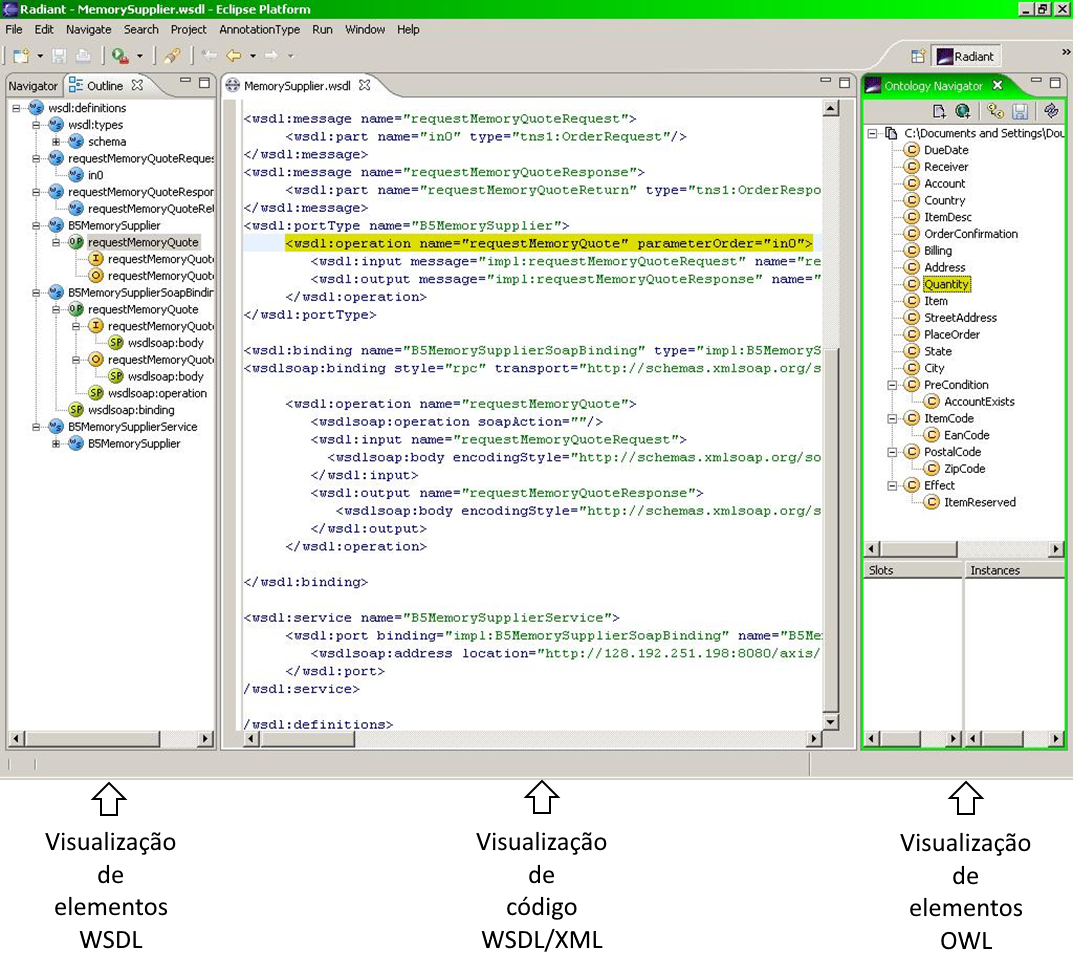
\includegraphics[scale=0.5]{2-fundamentacao-teorica/imagens/radiant3.png}
    \centering
    \caption[Interface gráfica de usuário da ferramenta Radiant.]{\textbf{Interface gráfica de usuário da ferramenta Radiant.}}
    \label{fig:radiant}
\end{figure}
\subsection{Iridescent}\label{2-fundamentacao-ferramentas-iridescent}

Iridescent~\cite{STAVROPOULOS-2013-Iridescent} é uma ferramenta \textit{standalone} que permite anotar descrições de serviços web de acordo com o padrão SAWSDL. As anotações são inseridas com base nas referências de termos de uma ontologia representada no formato OWL~\cite{W3C-2012-OWL}.

Por meio de uma interface gráfica de usuário, Iridescent permite que entidades identificadas na descrição de um serviço web sejam anotadas com os termos contidos na ontologia. A visualização de uma descrição de serviço web e uma ontologia ocorre por meio de uma representação visual no formato de árvore (\textit{tree-view}), semelhante ao \textit{plugin} Radiant~\cite{MILLER-VERMA-GOMADAM-SHETH-BREWER-2005-Radiant}.

Iridescent oferece recursos que automatizam parcialmente o processo de anotação semântica nos serviços web. A partir de um algoritmo de busca, conceitos de uma ontologia são sugeridos para os termos contidos em uma descrição de um serviço, servindo como um guia para o usuário. O usuário pode acatar ou não as sugestões da ferramenta. Iridescent também provê recursos para que os métodos \textit{Lifting Schema Mapping} e \textit{Lowering Schema Mapping} possam ser implementados e descritos no WSDL.

A utilização do recurso \textit{drag-and-drop} também auxilia o processo. O usuário pode arrastar elementos (conceitos) da representação visual de uma ontologia, do painel lateral direito, para um elemento WSDL presente no código disponibilizado pelo painel central. As anotações semânticas (SAWSDL) podem ser vistas diretamente no código WSDL/XML.

%O vínculo das anotações dos termos da ontologia com a descrição dos serviços web é realizado pela visualização do código WSDL/XML da descrição de serviço anotado semanticamente com a sintaxe SAWSDL~\cite{W3C-2007-SAWSDL}.

A \figurename~\ref{fig:iridescent} ilustra a interface gráfica de usuário de Radiant. Na lateral esquerda, encontram-se representados os elementos de uma ontologia. Na lateral direita, encontram-se representados os elementos WSDL. Finalmente, no centro, encontra-se a especificação WSDL anotada

\begin{figure}[h]
    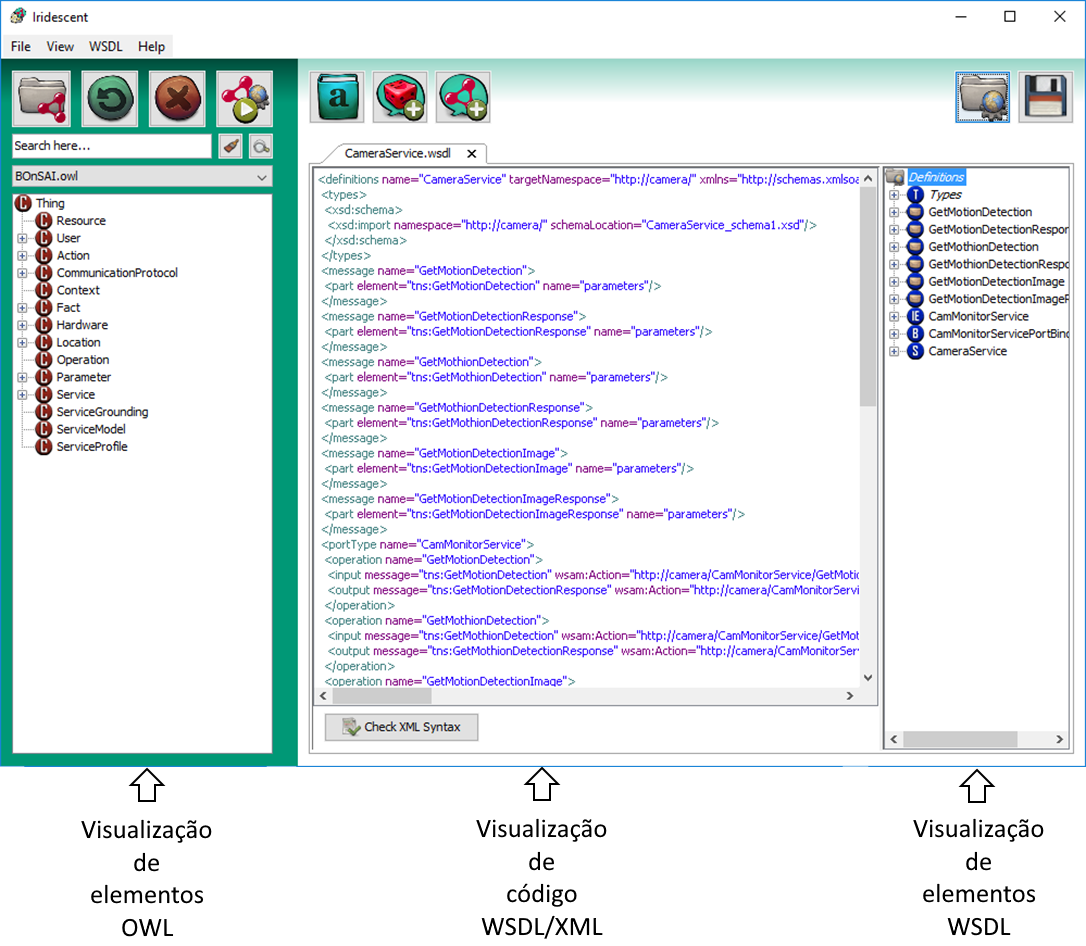
\includegraphics[scale=0.5]{2-fundamentacao-teorica/imagens/iridescent3.png}
    \centering
    \caption[Interface gráfica de usuário da ferramenta Iridescent.]{\textbf{Interface gráfica de usuário da ferramenta Iridescent.}}
    \label{fig:iridescent}
\end{figure}
\subsection{EasyWSDL \& EasySAWSDL}\label{2-fundamentacao-ferramentas-easywsdl}

EasyWSDL~\cite{EasyWSDL-2016} é uma biblioteca Java para suporte à leitura, à edição e à criação de documentos WSDL e XML Schema (XSD). EasyWSDL foi desenvolvida pelo \textit{OW2 Consortium}~\cite{OW2-2016-Site}, organização da comunidade \textit{open-source}, que tem como missão promover o desenvolvimento de aplicações \textit{middleware} e de negócio, plataformas de computação em nuvem, entre outras.

A arquitetura de EasyWSDL é extensível. Assim, a extensão EasySAWSDL~\cite{EasySAWSDL-2016} foi proposta para permitir a anotação de documentos WSDL segundo o padrão SAWSDL~\cite{W3C-2007-SAWSDL}. EasyWSDL fornece classes e métodos específicos para a criação e a manipulação de elementos de um documento WSDL, enquanto que EasySAWSDL fornece classes e métodos específicos para a anotação semântica. A manipulação de elementos WSDL e atributos SAWSDL são abstraídos por meio da linguagem de programação. A biblioteca provê métodos claros que permitem que desenvolvedores, familiarizados com a linguagem de programação Java, possam compreender e manipular mais facilmente o documento. Neste sentido, desenvolvedores não necessitam lidar diretamente com dados sintáticos das especificações WSDL e SAWSDL para a criação de serviços web semânticos.

%Por meio da arquitetura orientada a objetos da linguagem Java, EasyWSDL e sua extensão EasySAWSDL proveem um nível mais abstrato de construção e manipulação de elementos WSDL e atributos SAWSDL, dado que desenvolvedores de software normalmente estão mais familiarizados com linguagens de programação orientadas a objetos do que com os padrões WSDL e SAWSDL.

A \lstlistingname~\ref{lst:easywsdl} apresenta um exemplo de utilização da biblioteca EasySAWSDL para a anotação de uma especificação WSDL. As linhas 1 e 2 contém instruções para a leitura de um documento WSDL. O objeto \texttt{reader} é utilizado para a leitura de um documento WSDL, enquanto que o objeto \texttt{desc} é utilizado para o armazenamento de um documento WSDL. A linha 3 contém uma instrução necessária para a escrita de atributos SAWSDL. A linha 4 contém uma instrução para a leitura de uma descrição WSDL (objeto \texttt{desc}) por meio do escritor SAWSDL. A linha 5 contém uma instrução para obter um elemento WSDL (objeto \texttt{ele}) dado um identificador. Finalmente, a linha 6 contém uma instrução para adicionar um atributo \textit{Model Reference}, com o uso de uma URI de um conceito de uma ontologia.

%Refs da listagem:
% https://www.overleaf.com/learn/latex/Code_listing
% https://en.wikibooks.org/wiki/LaTeX/Source_Code_Listings
% http://texdoc.net/texmf-dist/doc/latex/listings/listings.pdf
\begin{lstlisting}[language=java,caption={[Exemplo de uso da biblioteca EasySAWSDL]\textbf{Exemplo de uso da biblioteca EasySAWSDL}.},label={lst:easywsdl}]
    WSDLReader reader = WSDLFactory.newInstance().newWSDLReader();
    Description desc = reader.read(new URL("http://grasews/svc.wsdl"));
    SAWSDLWriter writer = SAWSDLFactory.newInstance().newSAWSDLWriter();
    Document doc = writer.getDocument(desc);
    Element ele = doc.getElementById("elementId");
    ele.addModelReference(new URI("http://grasews.owl\#concept"));
\end{lstlisting}

%SAWSDLReader reader = SAWSDLFactory.newInstance().newSAWSDLReader();
\subsection{Avaliação Ferramental}\label{2-fundamentacao-ferramentas-avaliacao}

%As ferramentas Radiant, Iridescent e EasyWSDL/EasySAWSDL foram avaliadas segundo suas disponibilidades e suas usabilidades. A seguir são apresentadas características relevantes que nos auxiliaram durante esta avaliação.

%Radiant apresenta problemas quanto à sua disponibilidade. A distribuição de Radiant é realizada por meio de um plugin. A dependência do Eclipse para a sua utilização dificulta a sua adoção. O usuário deve ter um conhecimento prévio acerca da utilização do Eclipse. A configuração (instalação) do Eclipse e de Radiant no Eclipse são passos a mais que o usuário também deve realizar antes de iniciar o uso da ferramenta, o que pode contribuir para que a curva de aprendizagem de Radiant seja grande, i.e., iniciar o uso de Radiant pode requisitar um tempo adicional e não esperado. Adicionalmente, as distribuições de Radiant atualmente encontradas na Internet não são compatíveis com as versões mais recentes do Eclipse.

%Iridescent apresenta uma maior disponibilidade, visto que é uma ferramenta disponibilizada no formato \textit{standalone}. Tal formato não exige que seus usuários tenham um conhecimento prévio de outras ferramentas e tão pouco que dependam de outras distribuições. Neste sentido, a curva de aprendizagem de Iridescent é menor quando comparada com Radiant. Iridescent também apresentou erros (exceções não tratadas) durante o seu uso, o que impossibilitou sua utilização de forma fluente.

%Tanto Radiant quanto Iridescent requerem conhecimento técnico de XML/WSDL para que a anotação semântica possa ser realizada pelo usuário. Ambas ferramentas pressupõem que anotações semânticas devam ser inseridas diretamente no documento WSDL, mesmo que sejam facilitadas por meio de representações visuais dos elementos WSDL e dos elementos OWL e por recursos como \textit{drag-and-drop}.

%EasyWSDL e sua extensão EasySAWSDL foram facilmente encontradas. Por se tratar de uma biblioteca associada a uma linguagem de programação específica, esta solução possui usabilidade e aplicabilidade restritas.

%Por se tratar de uma biblioteca de desenvolvimento, EasyWSDL e EasySAWSDL também não exigem conhecimento prévio de outras ferramentas e integrações. Porém, exigem conhecimento de programação e da linguagem \textit{Java}, o que pode ser um grande desmotivador e fator bloqueante para o seu uso. Neste sentido, a biblioteca apresenta uma curva de aprendizagem maior que Radiant e Iridescent.

%A Tabela \ref{tab:formatos-distribuicao-ferramentas-disponiveis} resume os formatos de distribuição para as ferramentas apresentadas e avaliadas neste trabalho. A primeira coluna lista as ferramentas apresentadas neste trabalho. Já a segunda coluna lista os formatos de distribuição de cada ferramenta, conforme a primeira coluna.

%\begin{table}[h]
%    \setlength{\tabcolsep}{10pt} % Default value: 6pt
%    \renewcommand{\arraystretch}{2} % Default value: 1
%    \centering
%    \caption{Formatos de distribuição das ferramentas disponíveis.}
%    \label{tab:formatos-distribuicao-ferramentas-disponiveis}
%    \begin{tabular}{ | p{5cm} | p{7cm} | }
%        \hline  
%        \textbf{Ferramenta} & \textbf{Formato de Distribuição}
%        \\
%        \hline
%        {Radiant} & \textit{plugin}
%        \\
%        \hline
%        {Iridescent} & \textit{standalone}
%        \\
%        \hline
%        {EasyWSDL/EasySAWSDL} & {biblioteca de desenvolvimento (API)}
%        \\
%        \hline
%    \end{tabular}
%\end{table}

As ferramentas Radiant, Iridescent e EasyWSDL \& EasySAWSDL foram avaliadas segundo três critérios de usabilidade: i) facilidade de aprendizado, ii) maximização da produtividade e iii) minimização da taxa de erros. Facilidade de aprendizado refere-se ao esforço (tempo) necessário para aprender a utilizar a ferramenta e, portanto, atingir os resultados esperados. Quanto maior a facilidade de aprendizado, menor é a curva de aprendizagem. Maximização da produtividade refere-se à eficiência com a qual as ferramentas conseguem auxiliar seus usuários a atingirem os resultados esperados. Quanto maior a maximização da produtividade, maior é a eficiência. Finalmente, minimização da taxa de erros refere-se à facilidade com a qual exceções e fluxos não esperados executados por seus usuários. Quanto maior a minimização da taxa de erros, menor é a presença de erros.

Para realizar esta avaliação, utilizamos as três ferramentas para reproduzir parcialmente um conjunto de anotações semânticas desenvolvidas para diferentes serviços web na área de expressão gênica~\cite{GUARDIA-FARIAS-2017-SemantiSCo}. Cada diferente critério de usabilidade foi avaliado segundo uma classificação envolvendo níveis alto, médio e baixo.

No critério de facilidade de aprendizado, o \textit{plugin} Radiant foi avaliado em nível médio em razão da dificuldade associada à instalação e à configuração deste \textit{plugin}. Já a ferramenta Iridescent foi avaliada em nível alto neste critério por se tratar de uma ferramenta \textit{standalone} e, consequentemente, por não possuir dependências de outras ferramentas. Adicionalmente, Iridescent possui uma interface gráfica mais intuitiva quando comparado ao \textit{plugin} Radiant. Com isso, esta ferramenta apresentou uma maior facilidade de aprendizado em relação às demais. Finalmente, EasyWSDL \& EasySAWSDL foram avaliadas em nível baixo no critério de facilidade de aprendizado,
por se tratar de uma biblioteca de programação e, portanto, dependerem de conhecimento técnico prévio na linguagem de programação utilizada (Java).

Em relação ao critério de maximização da produtividade, as ferramentas Radiant e Iridescent foram avaliadas em nível médio, dado que, uma vez disponíveis, estas ferramentas permitiram a anotação semântica de forma simples. Entretanto, as anotações produzidas não são claramente percebidas dado que o usuário necessita visualizar a própria especificação WSDL para ter total compreensão das ações (anotações) realizadas. A biblioteca EasyWSDL \& EasySAWSDL foi avaliada em nível baixo, dada a necessidade de se criar um programa para permitir a anotação semântica de uma dada especificação WSDL.

%haja vista a sua interface gráfica não muito intuitiva 
%, devido à quantidade de passos e instruções necessárias para criar-se anotações semânticas em um documento WSDL.

Por fim, em relação ao critério de minimização da taxa de erros, Radiant e EasyWSDL \& EasySAWSDL não apresentaram erros durante sua utilização, portanto, sendo classificados em nível alto. Entretanto, Iridescent apresentou algumas falhas não tratadas ou pouco explicadas ao usuário, consequentemente, obtendo uma avaliação de nível médio.

A \tablename~\ref{tab:avaliacao-ferramentas-disponiveis} resume os critérios de usabilidade avaliados para cada ferramenta.

\begin{table}[ht!]
    \setlength{\tabcolsep}{10pt} % Default value: 6pt
    \renewcommand{\arraystretch}{1.5} % Default value: 1
    \centering
	\caption[Avaliação de usabilidade para as ferramentas disponíveis.]{\textbf{Avaliação de usabilidade para as ferramentas disponíveis.}}
	\label{tab:avaliacao-ferramentas-disponiveis}
	%\resizebox{\textwidth}{!}{
		\begin{tabular}{| >{\columncolor{Gray}}c | c | c | c | }
			\hline
            \rowcolor{Gray}
			{} & \textbf{Facilidade de} & \textbf{Maximização da} & \textbf{Minimização da}
			\\
            \rowcolor{Gray}
			\multirow{-1.5}{*}[3px]{\textbf{Ferramenta}} & \textbf{aprendizado} & \textbf{produtividade} & \textbf{taxa de erros}
			\\
			\hline
			\textbf{Radiant} & {Médio} & {Médio} & \textcolor{blue}{Alto}
			\\
            \hline
			\textbf{Iridescent} & \textcolor{blue}{Alto} & {Médio} & {Médio}
			\\ 
            \hline
			\textbf{EasySAWSDL} & \textcolor{red}{Baixo} & \textcolor{red}{Baixo} & \textcolor{blue}{Alto}
			\\
            \hline
		\end{tabular}
	%}
\end{table}
%\input{2-fundamentacao-teorica/2.5.4-owl-s-editor}